%%%%%%%%%%%%%%%%%%%%%%%%%%%%%%%%%%%%%%%
% Header                              %
%%%%%%%%%%%%%%%%%%%%%%%%%%%%%%%%%%%%%%%
% 
% Revisions: 2017-12-12 Martin Raedel <martin.raedel@dlr.de>
%                       Initial draft
%               
% Contact:   Martin Raedel,  martin.raedel@dlr.de
%            DLR Composite Structures and Adaptive Systems
%          
%                                 __/|__
%                                /_/_/_/  
%            www.dlr.de/fa/en      |/ DLR
% 
%%%%%%%%%%%%%%%%%%%%%%%%%%%%%%%%%%%%%%%
% Content                             %
%%%%%%%%%%%%%%%%%%%%%%%%%%%%%%%%%%%%%%%

% Figs
\begin{subfigure}{0.49\linewidth}
  % Length
  \setlength{\figwidth}{\linewidth}
  % Figure
  \centering
  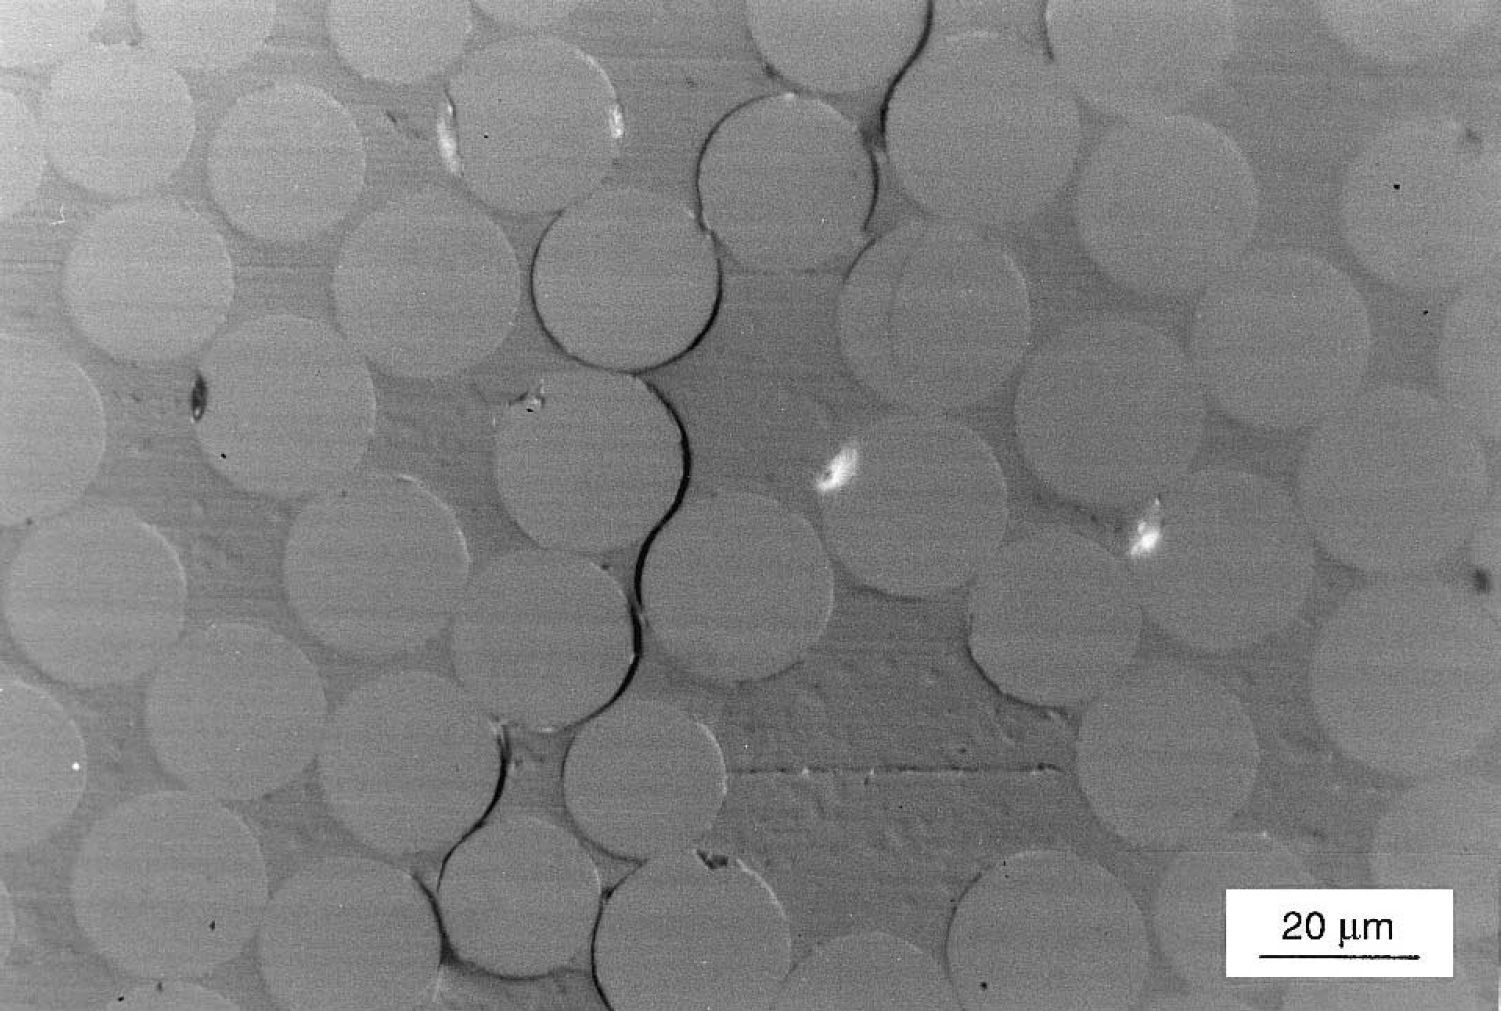
\includegraphics[width=\figwidth,height=\figheight,keepaspectratio]{Exp_RVE_GamstedtEK_I_Debond}
  \caption{Debond}%
  \label{fig:Exp:RVE:GamstedtEK:Debond}
\end{subfigure}%
\hfill
\begin{subfigure}{0.49\linewidth}
  % Length
  \setlength{\figwidth}{\linewidth}
  % Figure
  \centering
  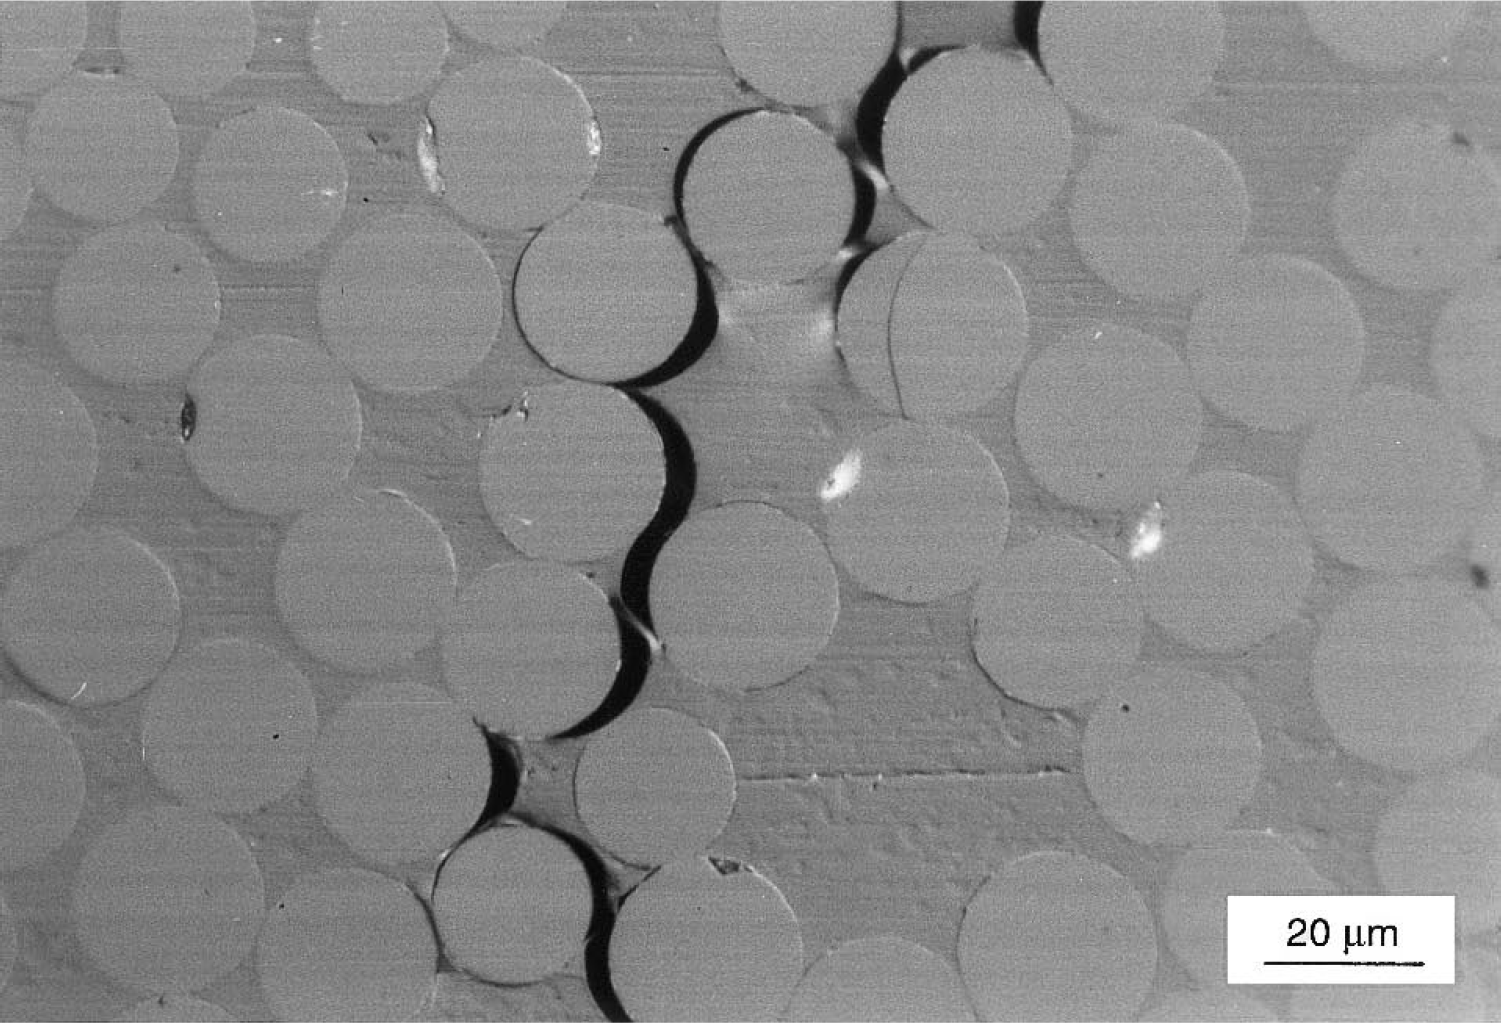
\includegraphics[width=\figwidth,height=\figheight,keepaspectratio]{Exp_RVE_GamstedtEK_II_TransverseCrack}
  \caption{Transverse crack}%
  \label{fig:Exp:RVE:GamstedtEK:TransverseCrack}
\end{subfigure}%